\section{OpenVAS Interface}

\sectionframe


% \frame{
% 	\frametitle{The most important thing\: The Feed}
% 		\begin{columns}[T,onlytextwidth,c]
%         \begin{column}{0.3\textwidth}
% 			\begin{itemize}
% 				\item This is the most important aspect of the tool: without it nothing will work
% 				\item Will take a lot of time to sync
% 				\item Every startup it tries to sync
% 			\end{itemize}
% 		\end{column}
% 		\begin{column}{0.6\textwidth} % Give the column a width here
% 			\centering
% 			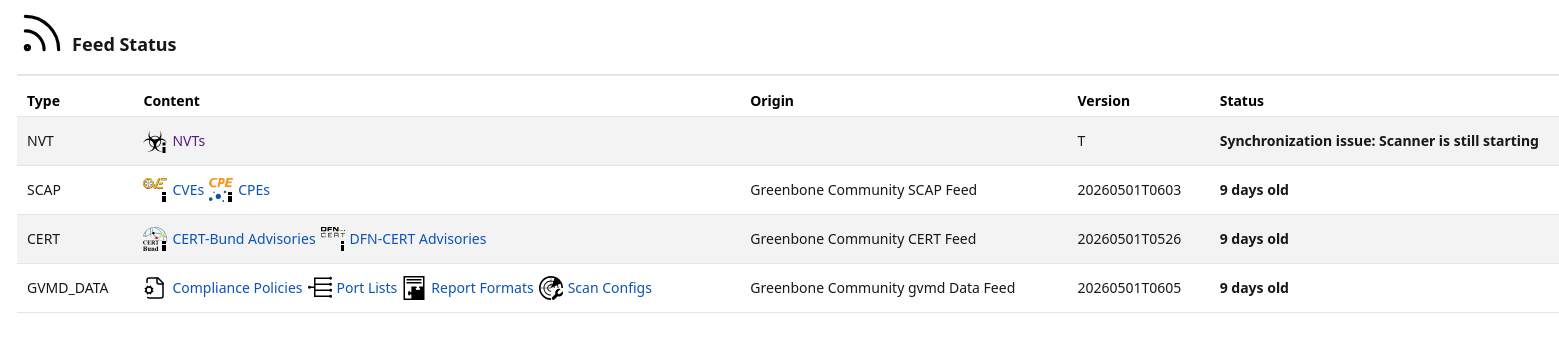
\includegraphics[width=\textwidth]{images/openvas_feed.png}
% 		\end{column}
%     \end{columns}
% }

\frame{
	\frametitle{Ports interface}
	\begin{center}
		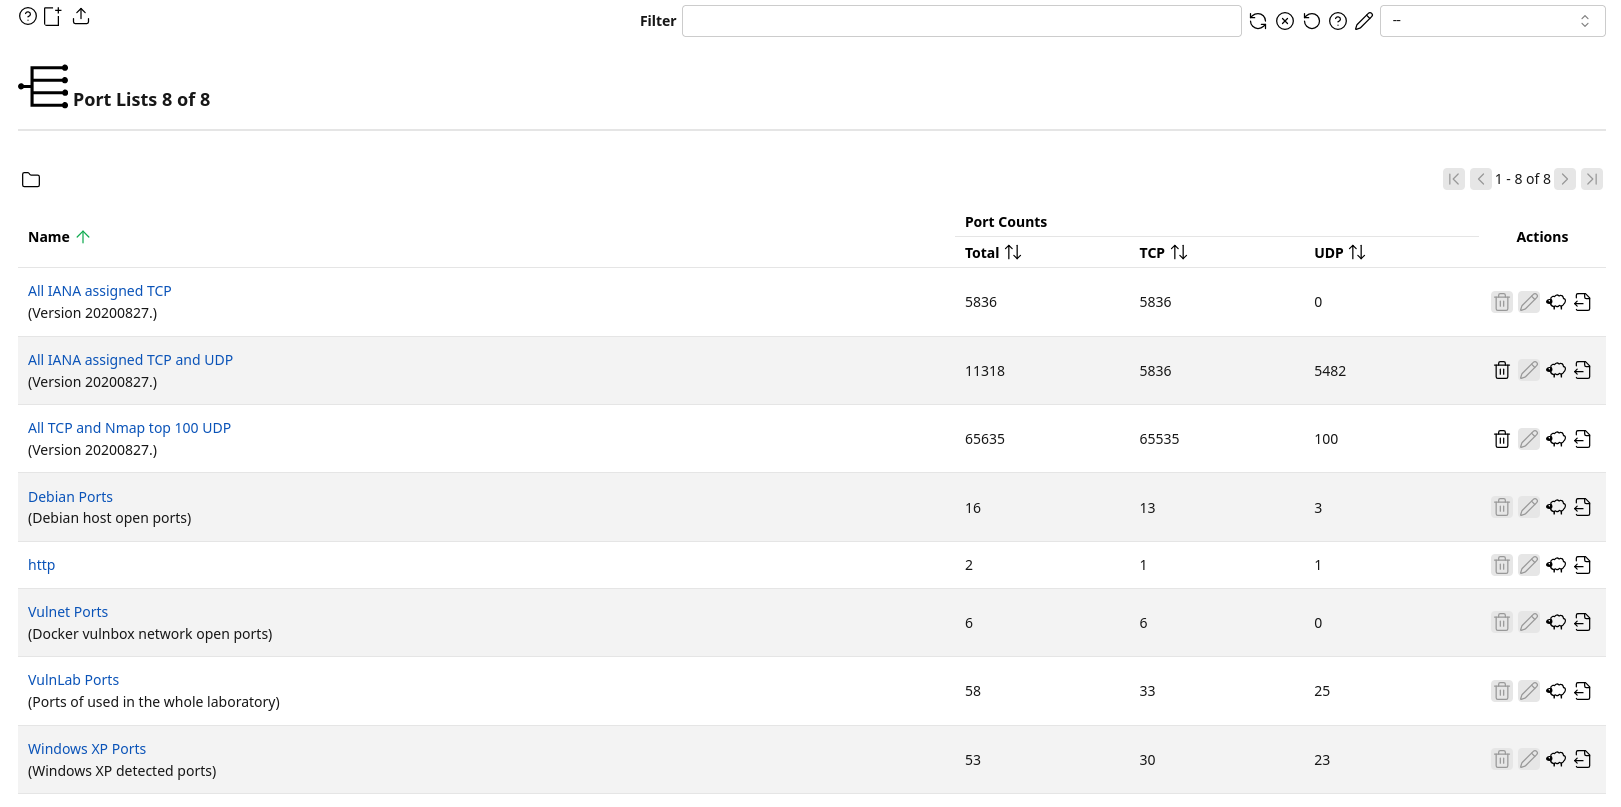
\includegraphics[width=0.9\textwidth]{images/openvas_ports_interface1.png}
	\end{center}

}

\frame{
	\frametitle{Port creation}
	\begin{columns}[T,onlytextwidth]
		\begin{column}{0.4\textwidth}
		\begin{itemize}
			\item Ports are expressed in its own format
			\item e.g. T:1-1024, 4500, U:1-100, 1023
		\end{itemize}
		\end{column}

       \begin{column}{0.6\textwidth}
           \centering
           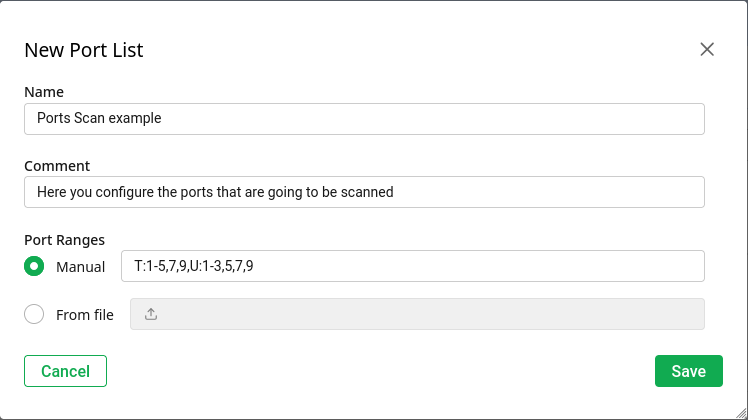
\includegraphics[width=\textwidth]{images/openvas_ports_scan1.png}
       \end{column}
    \end{columns}
}


\frame{
	\frametitle{Credentials for target access}
	\begin{columns}[T,onlytextwidth]
		\begin{column}{0.4\textwidth}
		\begin{itemize}
			\item You may also give the appliance the target credentials to have a more in-depth scan.
			\item It may improve accuracy since it scans more deeply, looking also at config files.
		\end{itemize}
		\end{column}

       \begin{column}{0.6\textwidth}
           \centering
           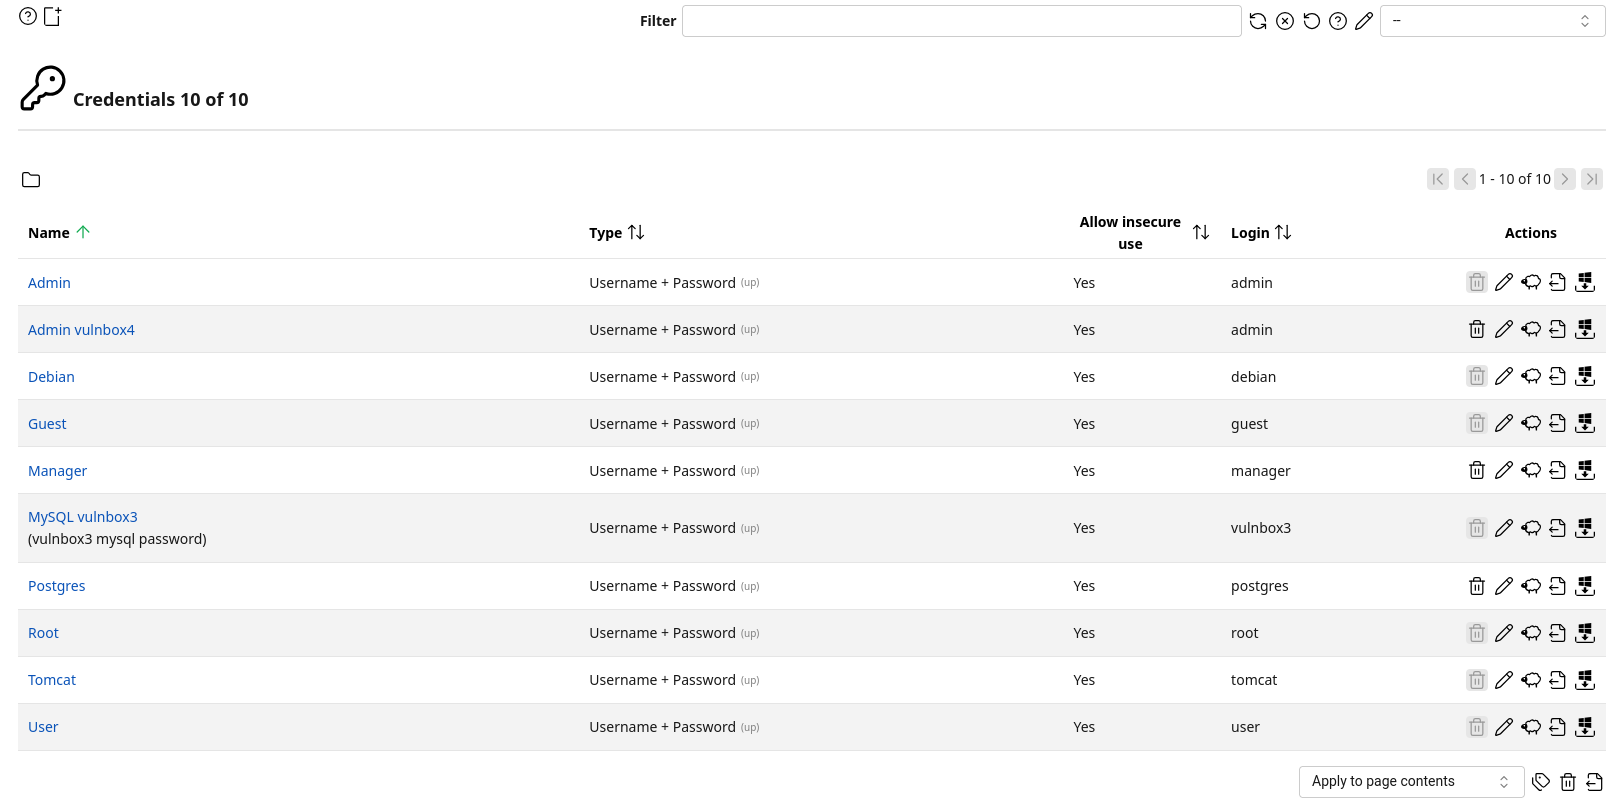
\includegraphics[width=\textwidth]{images/openvas_credentials1.png}
       \end{column}
    \end{columns}
}

\frame{
	\frametitle{Set scan credentials (for deeper scans)}
	\begin{columns}[T,onlytextwidth]
		\begin{column}{0.4\textwidth}
		   \centering
           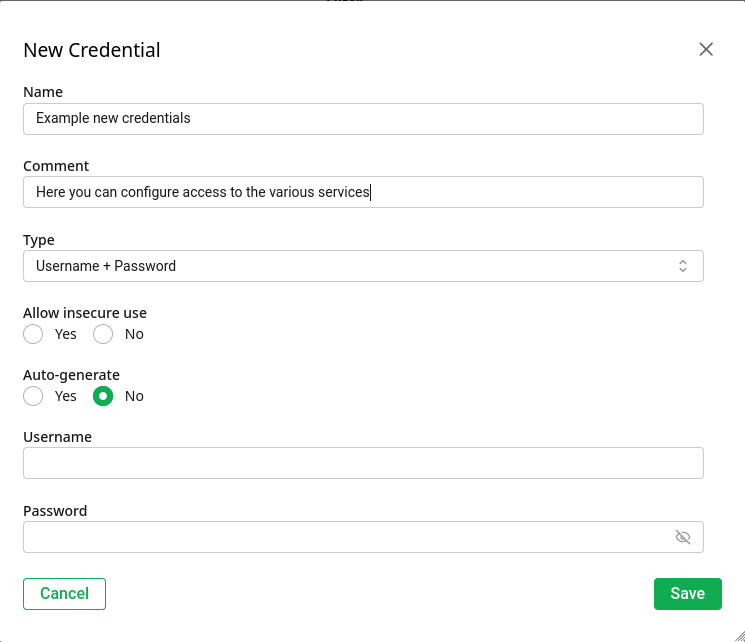
\includegraphics[width=\textwidth]{images/openvas_new_credentials1.png}
		\end{column}

       \begin{column}{0.4\textwidth}
           \centering
           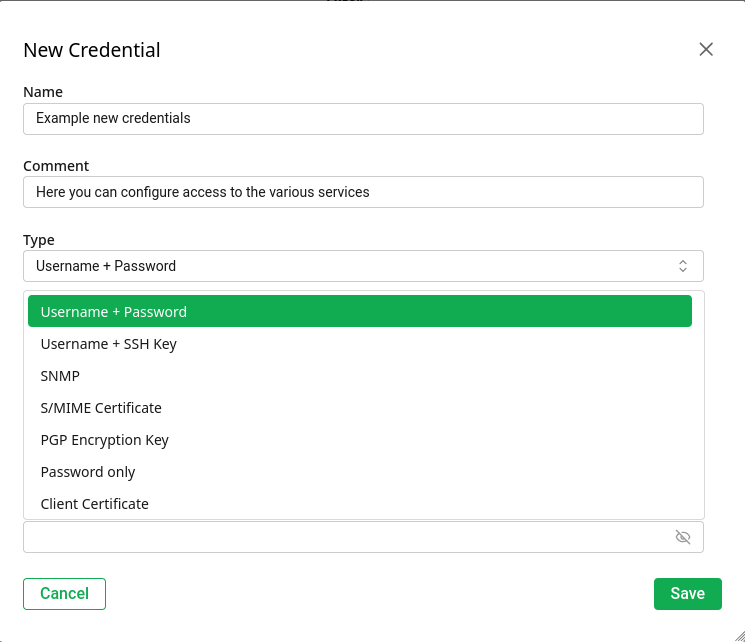
\includegraphics[width=\textwidth]{images/openvas_new_credentials2.png}
       \end{column}
    \end{columns}

}


\frame{
	\frametitle{Target interface}
	\begin{center}
		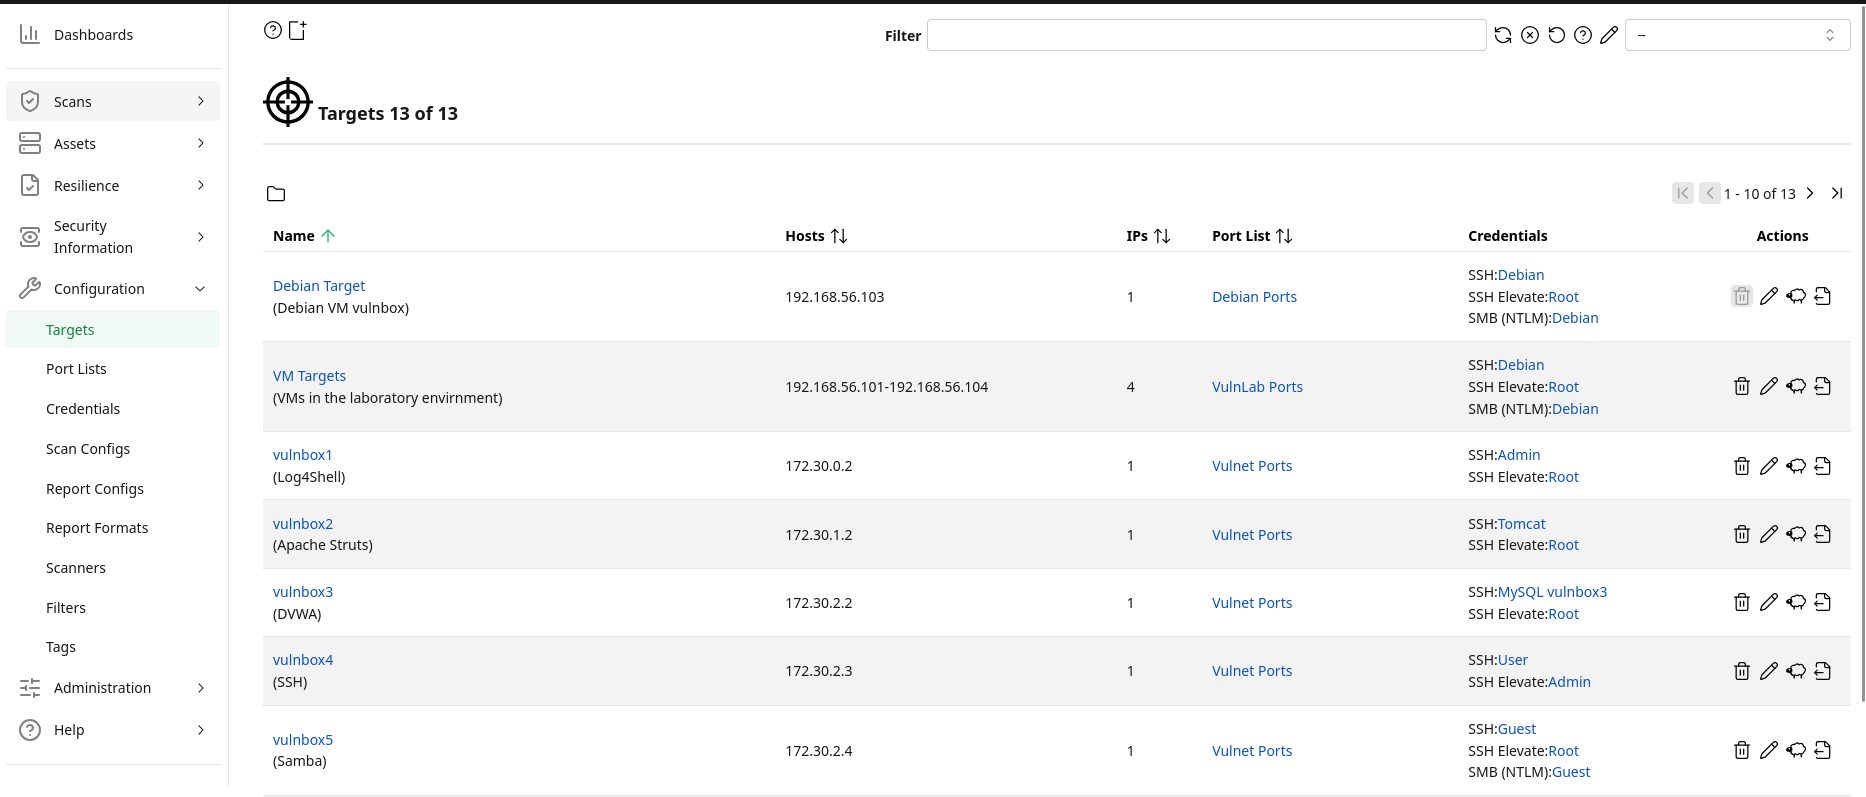
\includegraphics[width=0.9\textwidth]{images/openvas_conftargets.png}
	\end{center}

}

\frame{
	\frametitle{Target creation}
	\begin{columns}[T,onlytextwidth]
       \begin{column}{0.4\textwidth}
        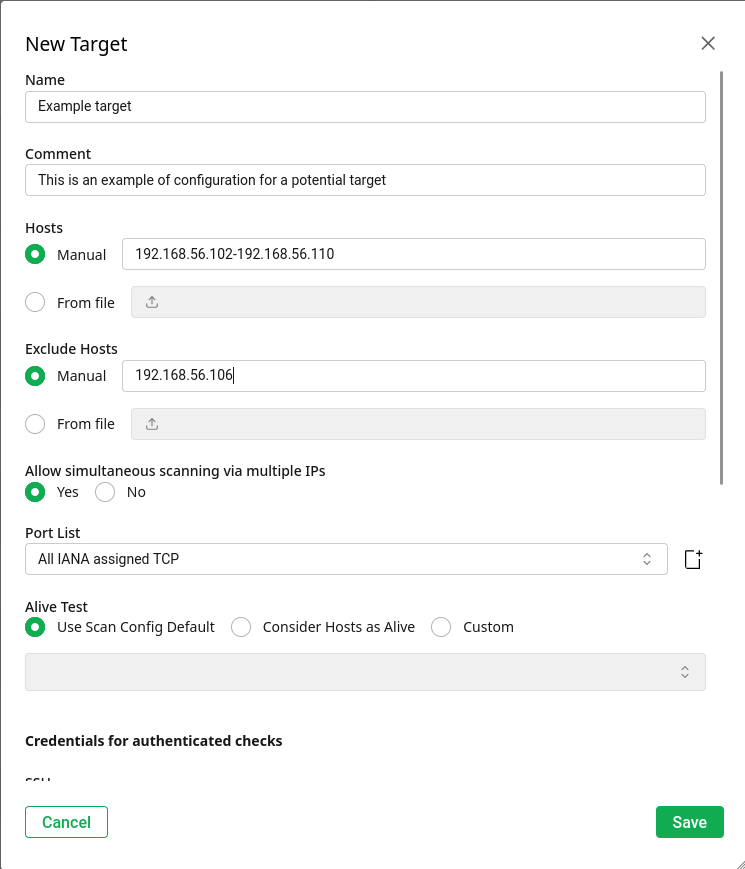
\includegraphics[width=\textwidth]{images/openvas_newtarget1.png}
       \end{column}
       \begin{column}{0.4\textwidth}
           \centering
           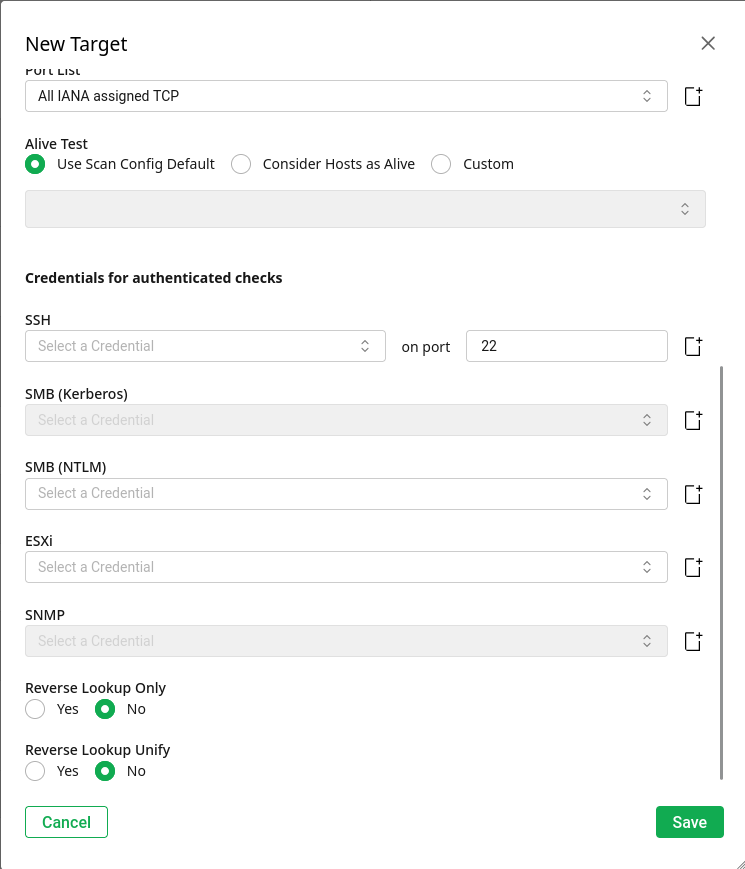
\includegraphics[width=\textwidth]{images/openvas_newtarget2.png}
       \end{column}
    \end{columns}
}

\frame{
	\frametitle{Scan configs}
	\begin{center}
		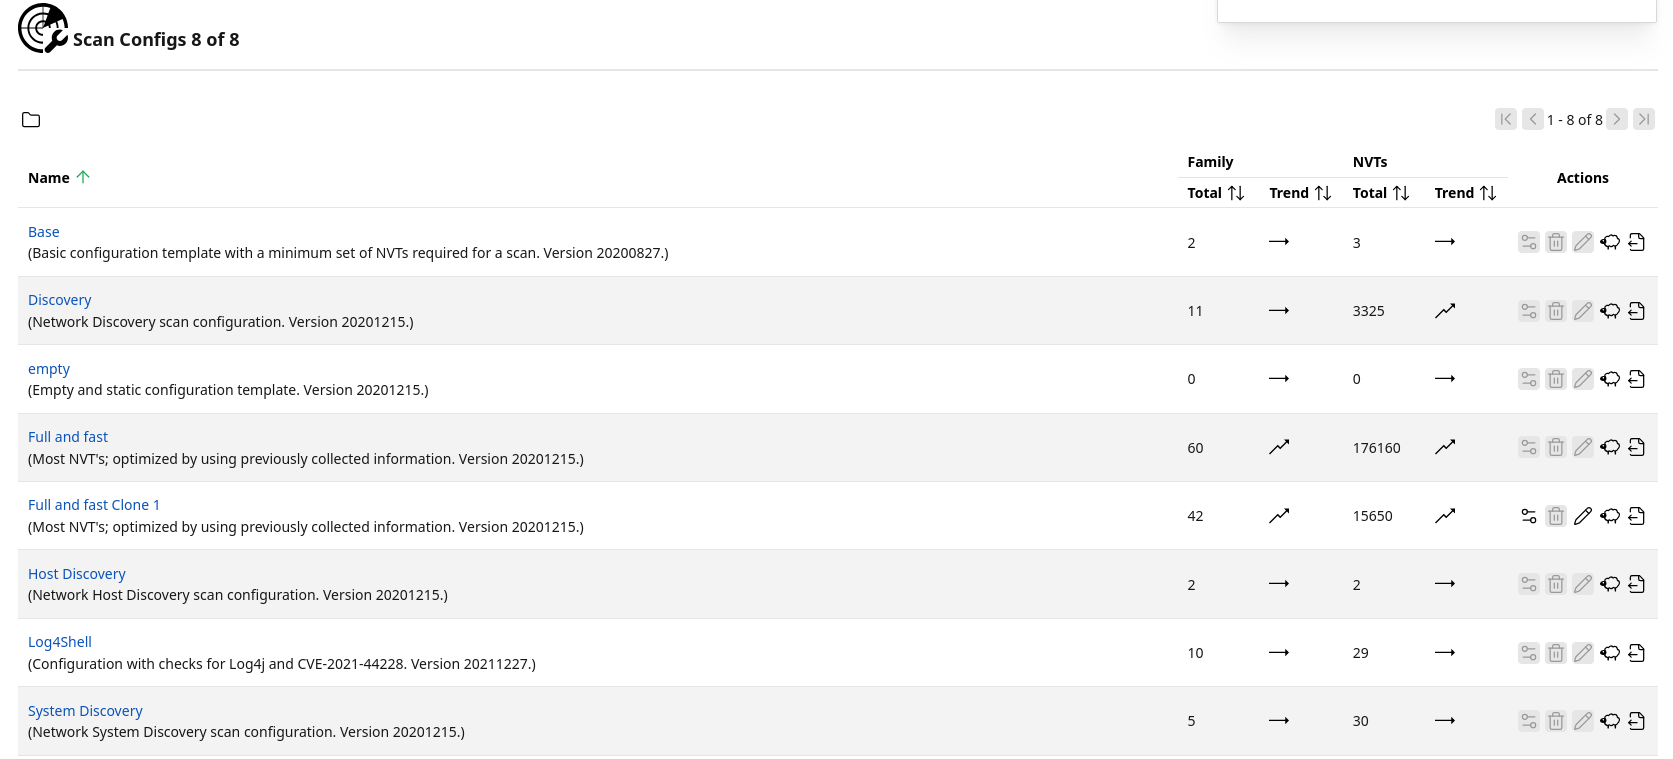
\includegraphics[width=0.9\textwidth]{images/openvas_scan_config1.png}
	\end{center}
}
\frame{
	\frametitle{Scan configs}
	% \begin{center}
	% 	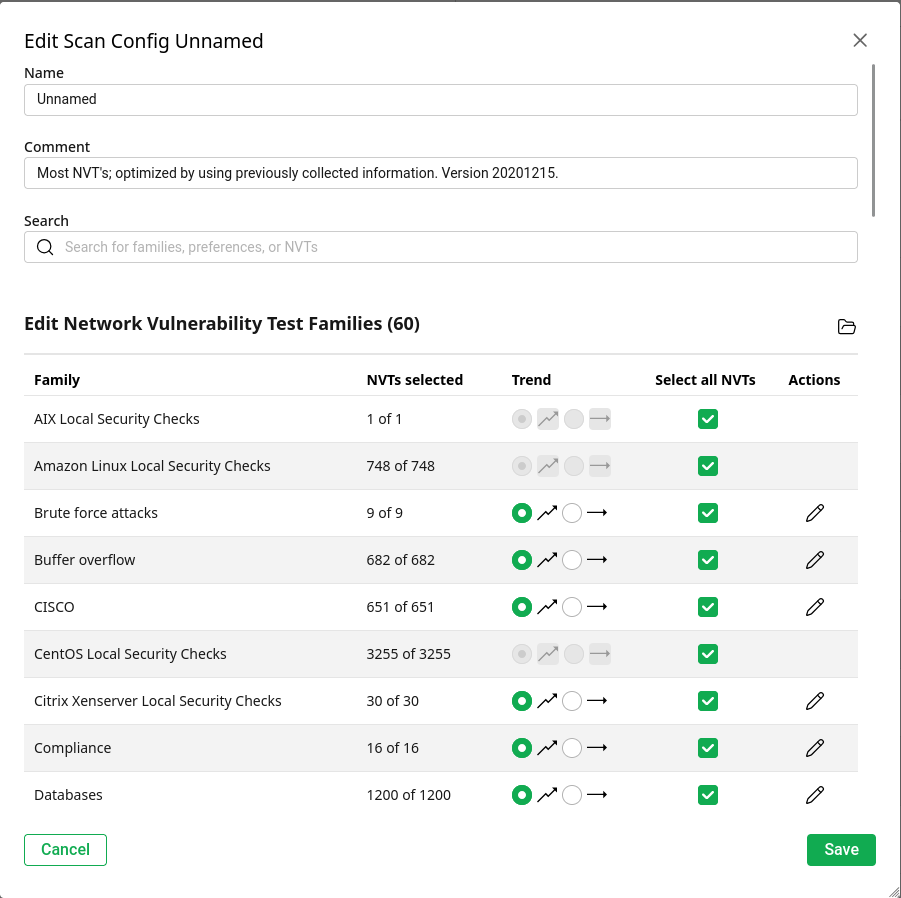
\includegraphics[width=0.5\textwidth]{images/openvas_scan_config2.png}
	% \end{center}

	\begin{columns}[T,onlytextwidth]
       \begin{column}{0.4\textwidth}
		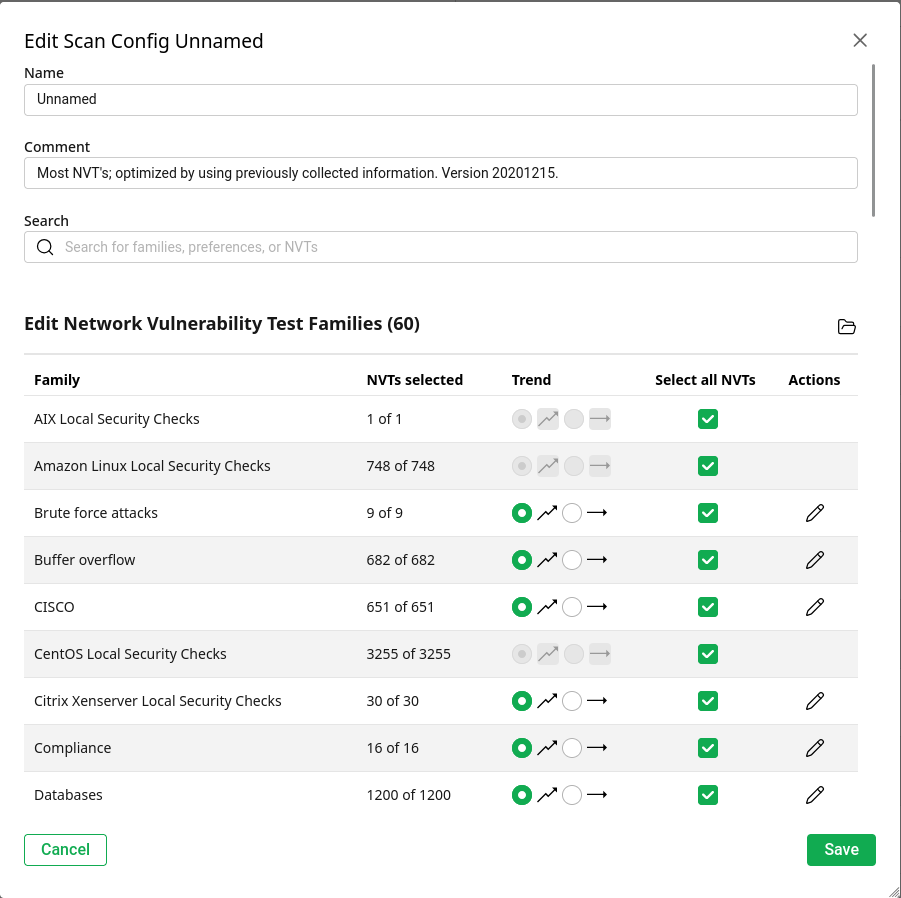
\includegraphics[width=\textwidth]{images/openvas_scan_config2.png}
       \end{column}
       \begin{column}{0.4\textwidth}
           \centering
		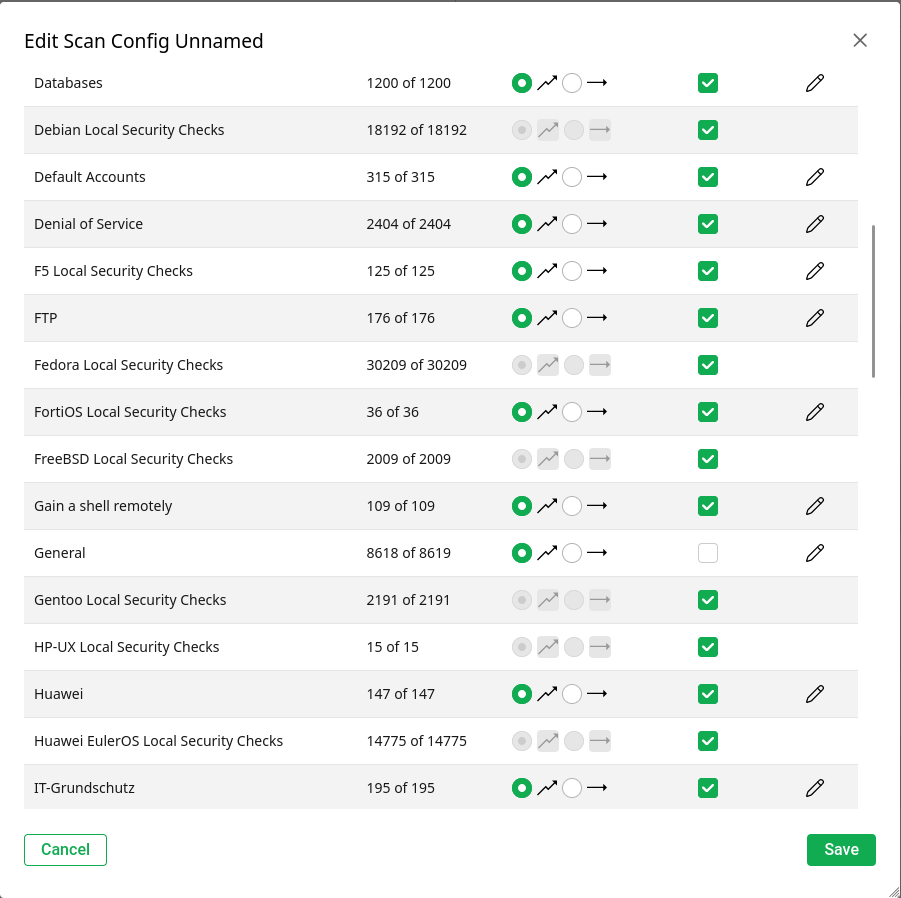
\includegraphics[width=\textwidth]{images/openvas_scan_config3.png}
       \end{column}
    \end{columns}
}
% \frame{
% 	\frametitle{Scan configs}
% 	\begin{center}
% 		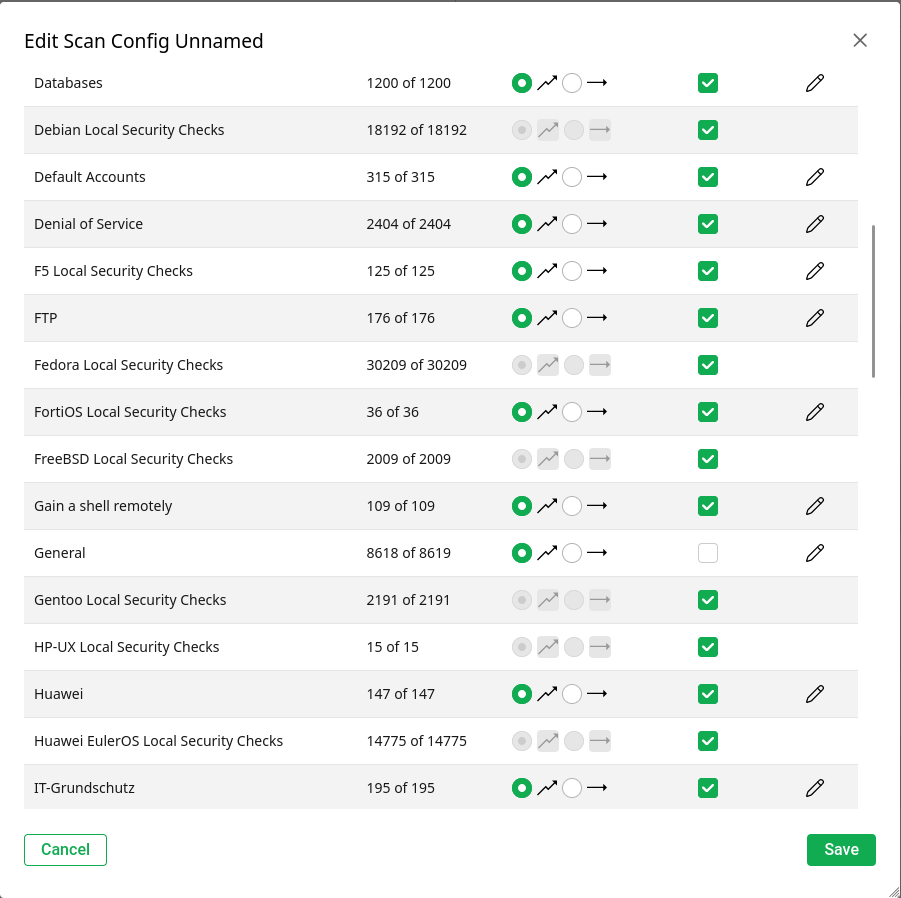
\includegraphics[width=0.5\textwidth]{images/openvas_scan_config3.png}
% 	\end{center}
% }

\frame{
	\frametitle{Scan interface}
	\begin{center}
		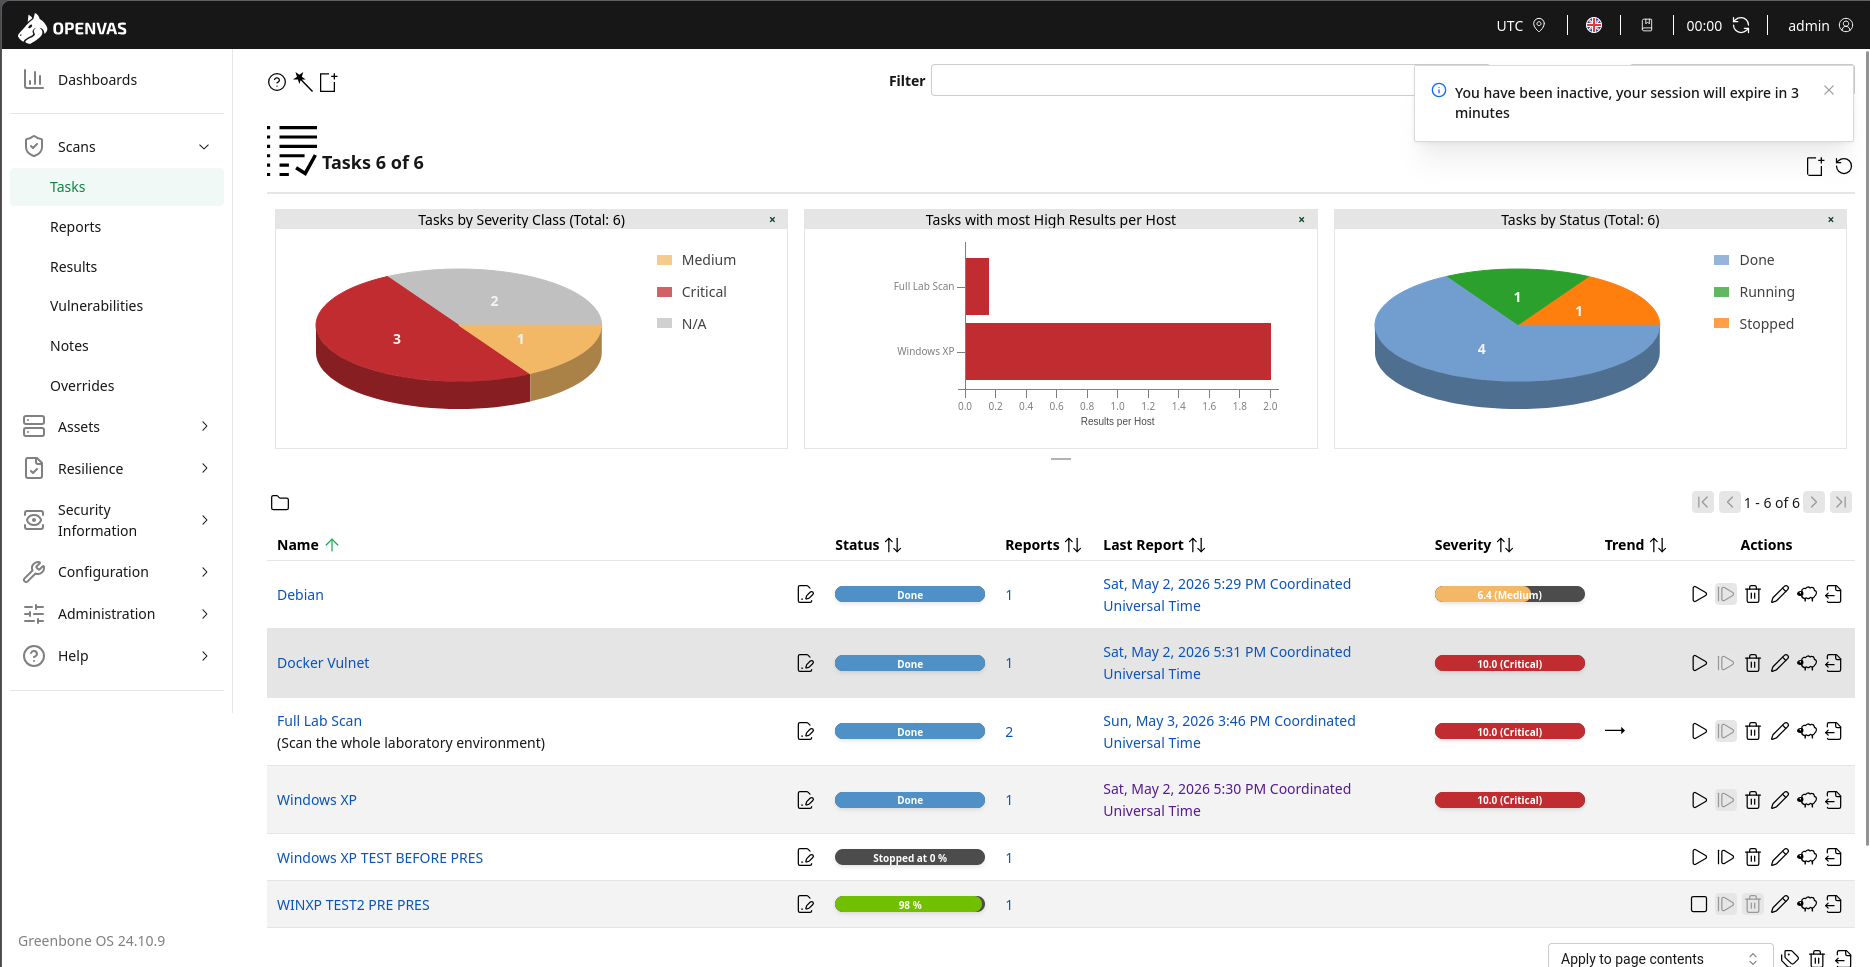
\includegraphics[width=0.9\textwidth]{images/openvas_scan_interface1.png}
	\end{center}

	%\begin{columns}[T,onlytextwidth]
    %    \begin{column}{0.4\textwidth}
    %        These are the 3 VMs:
    %        \begin{itemize}
    %            \item OPENVAS-FREE-24.10.9-VirtualBox
    %            \item Debian
    %            \item Windows XP
    %        \end{itemize}
    %        Configure the Network \underline{of all of them}
    %        by selecting the \textbf{Host-only Adapter} as network adapter 
    %        and choosing the network you created in the previous step.
    %    \end{column}
    %    \begin{column}{0.6\textwidth}
    %        \centering
    %        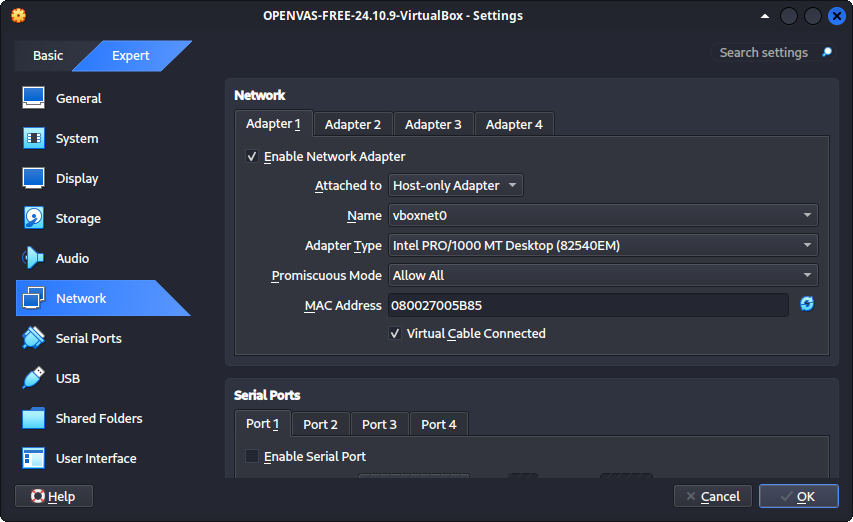
\includegraphics[width=\textwidth]{images/net_setup_3.png}
    %    \end{column}
    %\end{columns}
}

\frame{
	\frametitle{Task creation}
	\begin{columns}[T,onlytextwidth]
       \begin{column}{0.4\textwidth}
        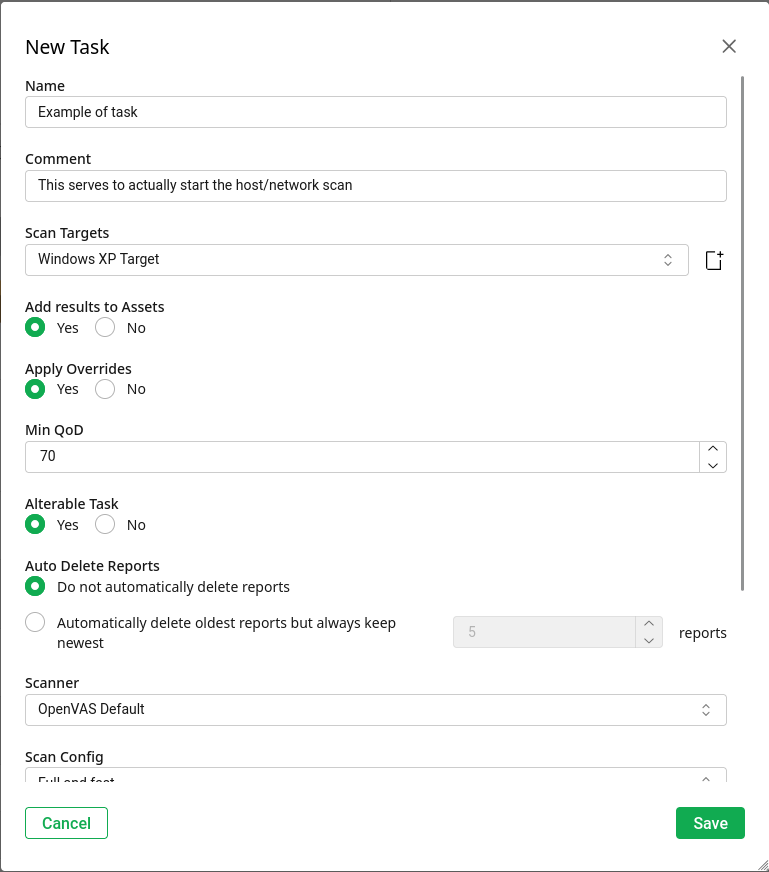
\includegraphics[width=\textwidth]{images/openvas_task_creation1.png}
       \end{column}
       \begin{column}{0.4\textwidth}
           \centering
           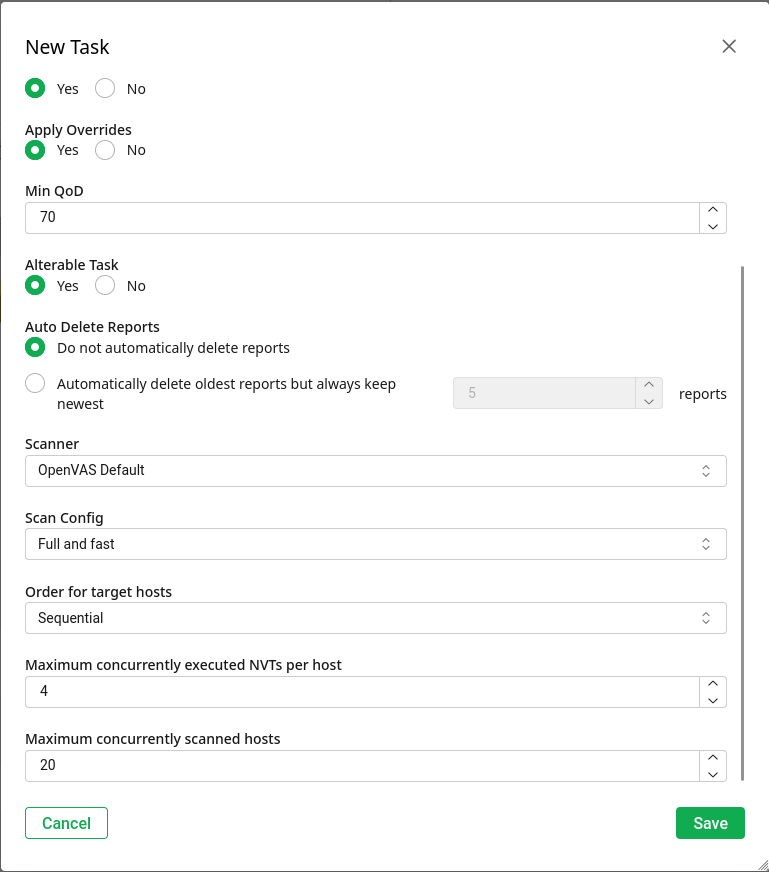
\includegraphics[width=\textwidth]{images/openvas_task_creation2.png}
       \end{column}
    \end{columns}
}





% \frame{
% 	\frametitle{Exercise: Scan for services on Windows XP}
% 	Try and start a scan for Windows XP on port 21 using Full and Fast preset
% 	\begin{itemize}
% 		\item Create the port record
% 		\item Create host record (should be 192.168.56.10x depending on the IP)
% 		\item Create a new task (remember to make it adjustable, otherwise you have to recreate it from scratch), remember to schedule it
% 	\end{itemize}

% }

\frame{
	\frametitle{Assets: Operating Systems}
	\begin{center}
		\includegraphics[width=0.9\textwidth]{images/openvas_asset_OS.png}
	\end{center}

}
\frame{
	\frametitle{Assets: TLS Certificates}
	\begin{center}
		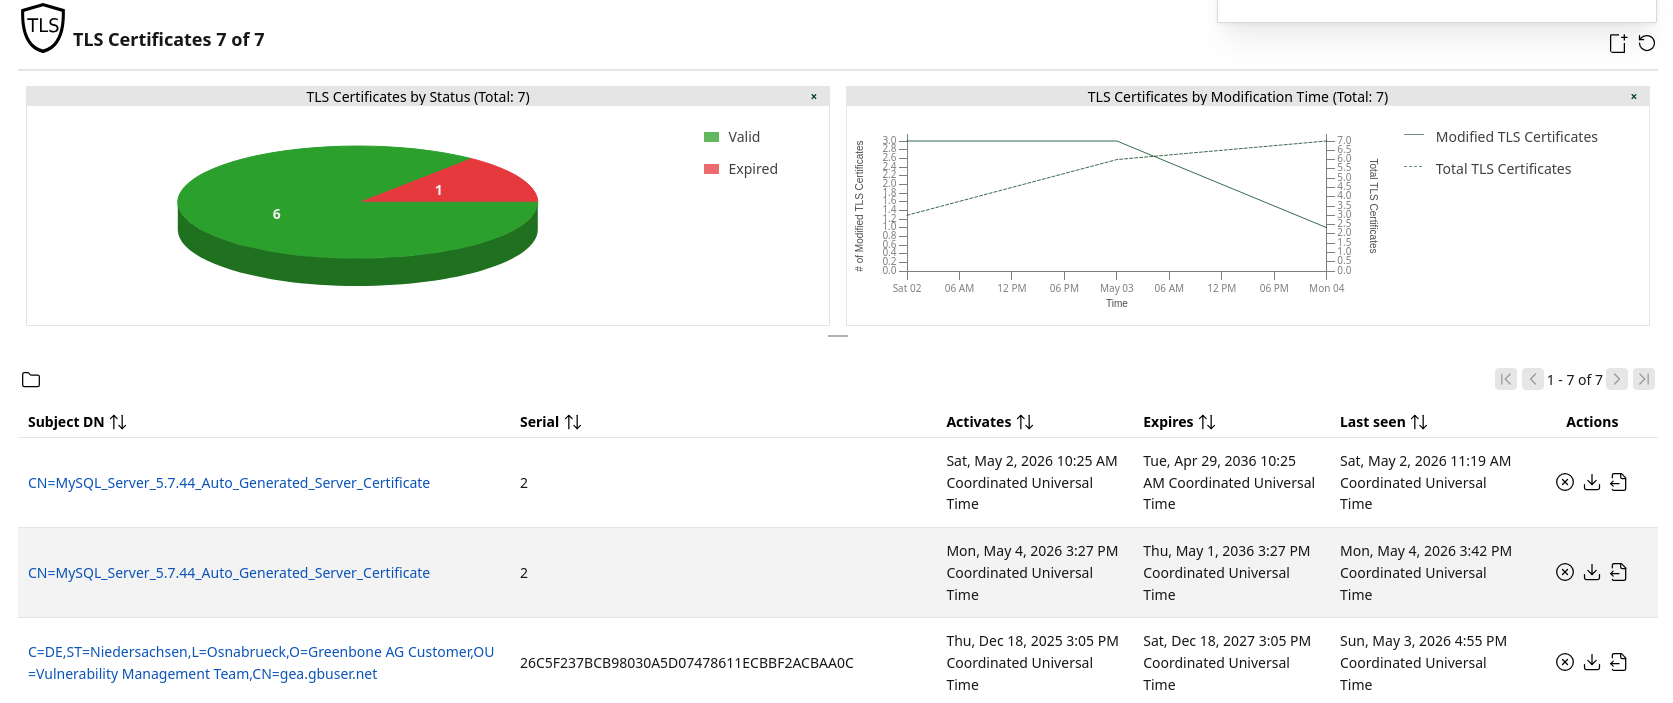
\includegraphics[width=0.9\textwidth]{images/openvas_asset_tls.png}
	\end{center}

}

\frame{
	\frametitle{Exercise: Scan for services on Windows XP}
	Try and start a scan for Windows XP on port 21 using Full and Fast preset
	\begin{itemize}
		\item Create the port record
		\item Create host record (should be 192.168.56.10x depending on the IP)
		\item Create a new task (remember to make it adjustable, otherwise you have to recreate it from scratch), remember to schedule it
	\end{itemize}

}



\frame{
	\frametitle{Reports}
	\begin{columns}[T,onlytextwidth]
		\begin{column}{0.3\textwidth}
		\begin{itemize}
			\item After a scan has been done, a report will be created citing everyting the tool founds.
			\item You can also see the severity of the Vulnerability he finds
		\end{itemize}
		\end{column}

       \begin{column}{0.6\textwidth}
           \centering
           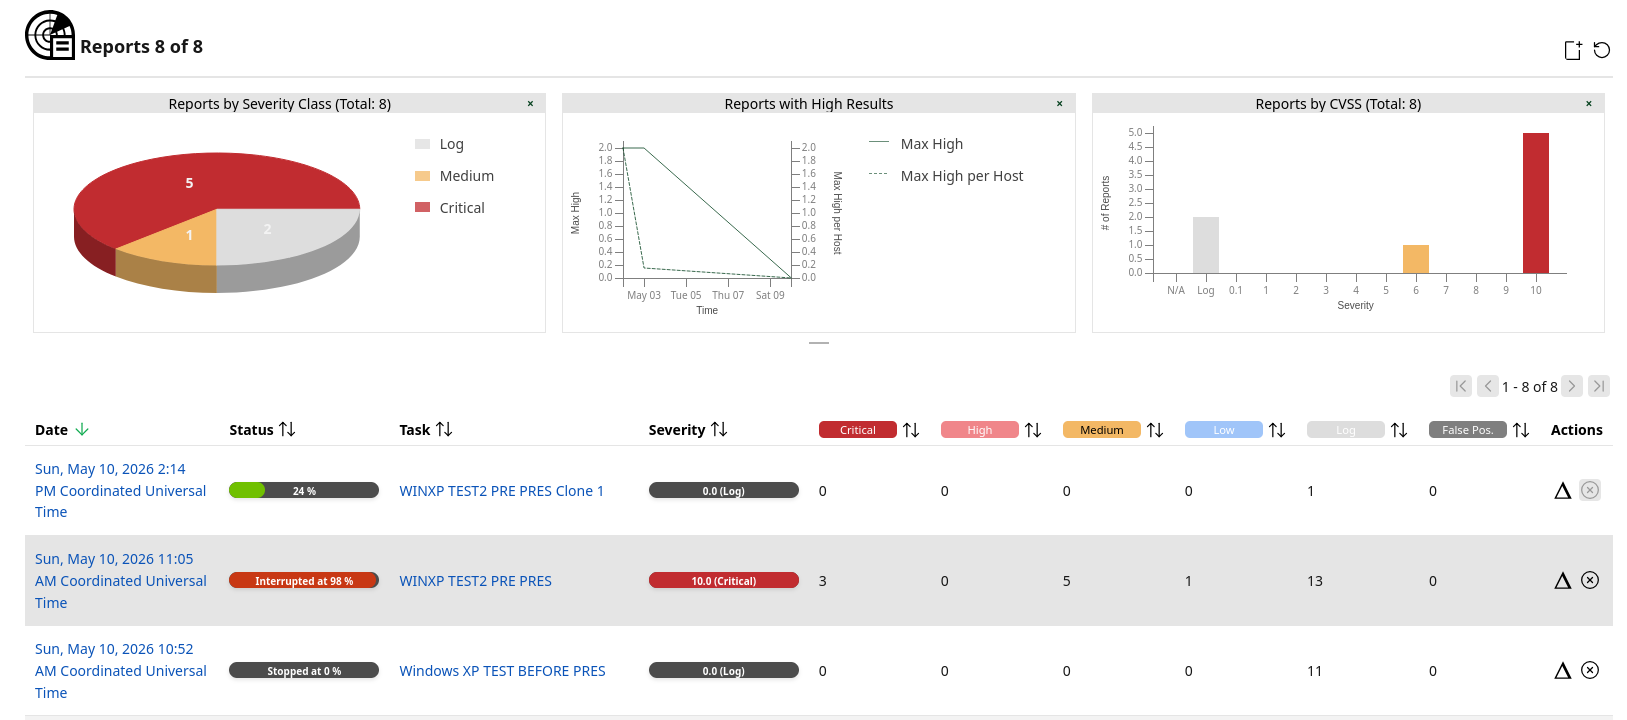
\includegraphics[width=\textwidth]{images/openvas_report.png}
       \end{column}
    \end{columns}
}

\frame{
	\frametitle{Results}
		\begin{columns}[T,onlytextwidth]
		\begin{column}{0.3\textwidth}
		\begin{itemize}
			\item Here you will see the results sorted by severity across all scans 
		\end{itemize}
		\end{column}

       \begin{column}{0.65\textwidth}
           \centering
           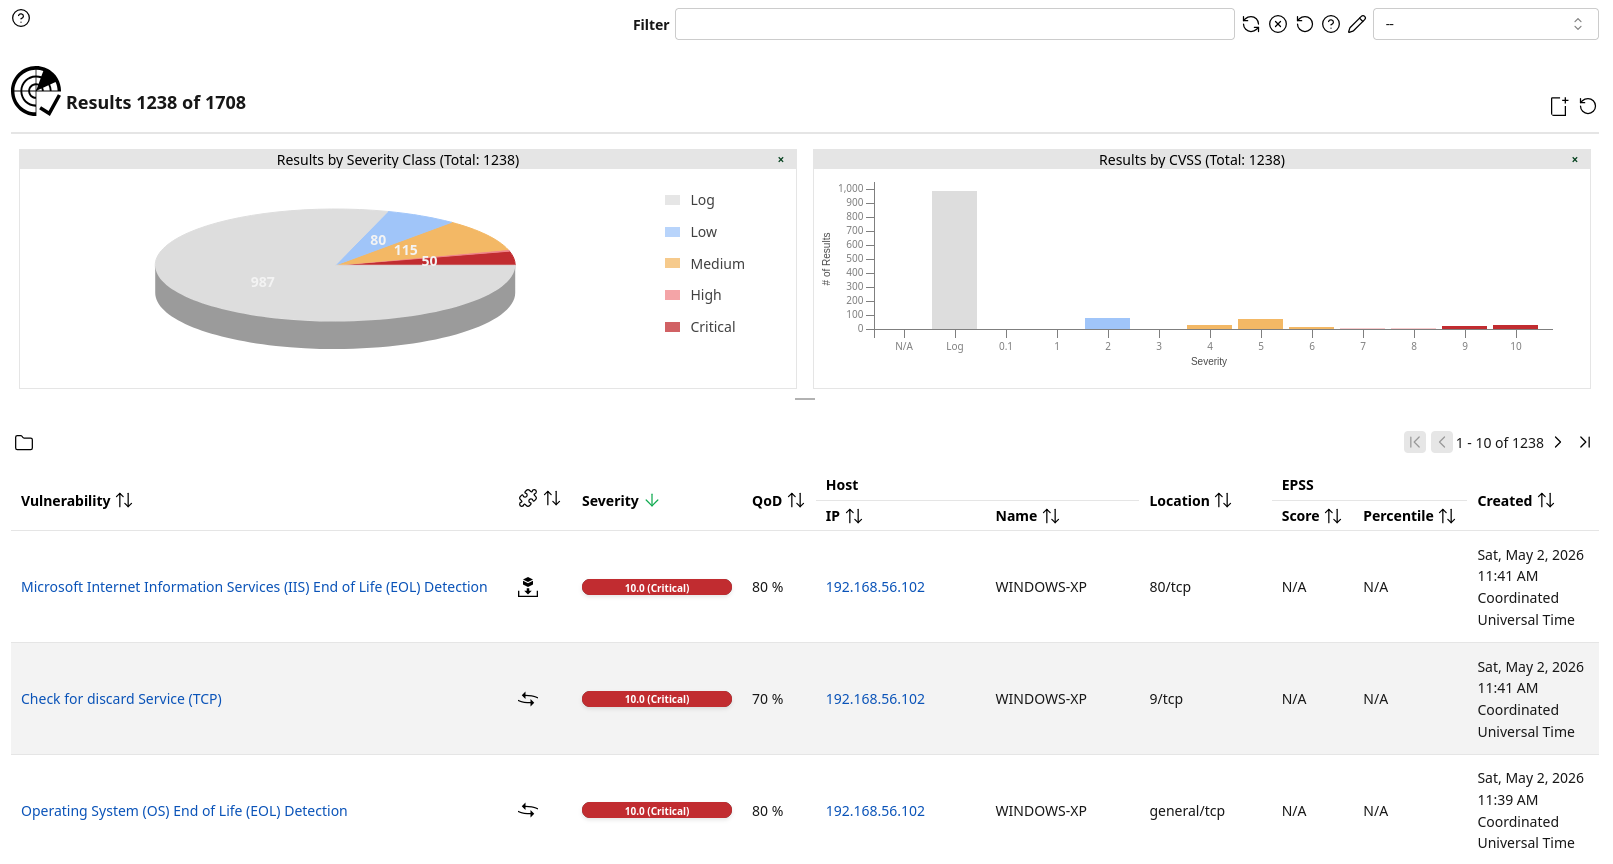
\includegraphics[width=\textwidth]{images/openvas_results.png}
       \end{column}
    \end{columns}
}


% TODO: Creare esercizio configuration scan configs e ripetere la scansione
% TODO: Spiegare differenze tra scan configs
% TODO: FIX ORDER